%!TEX root = ../../main.tex


\begin{figure}[!htbp]
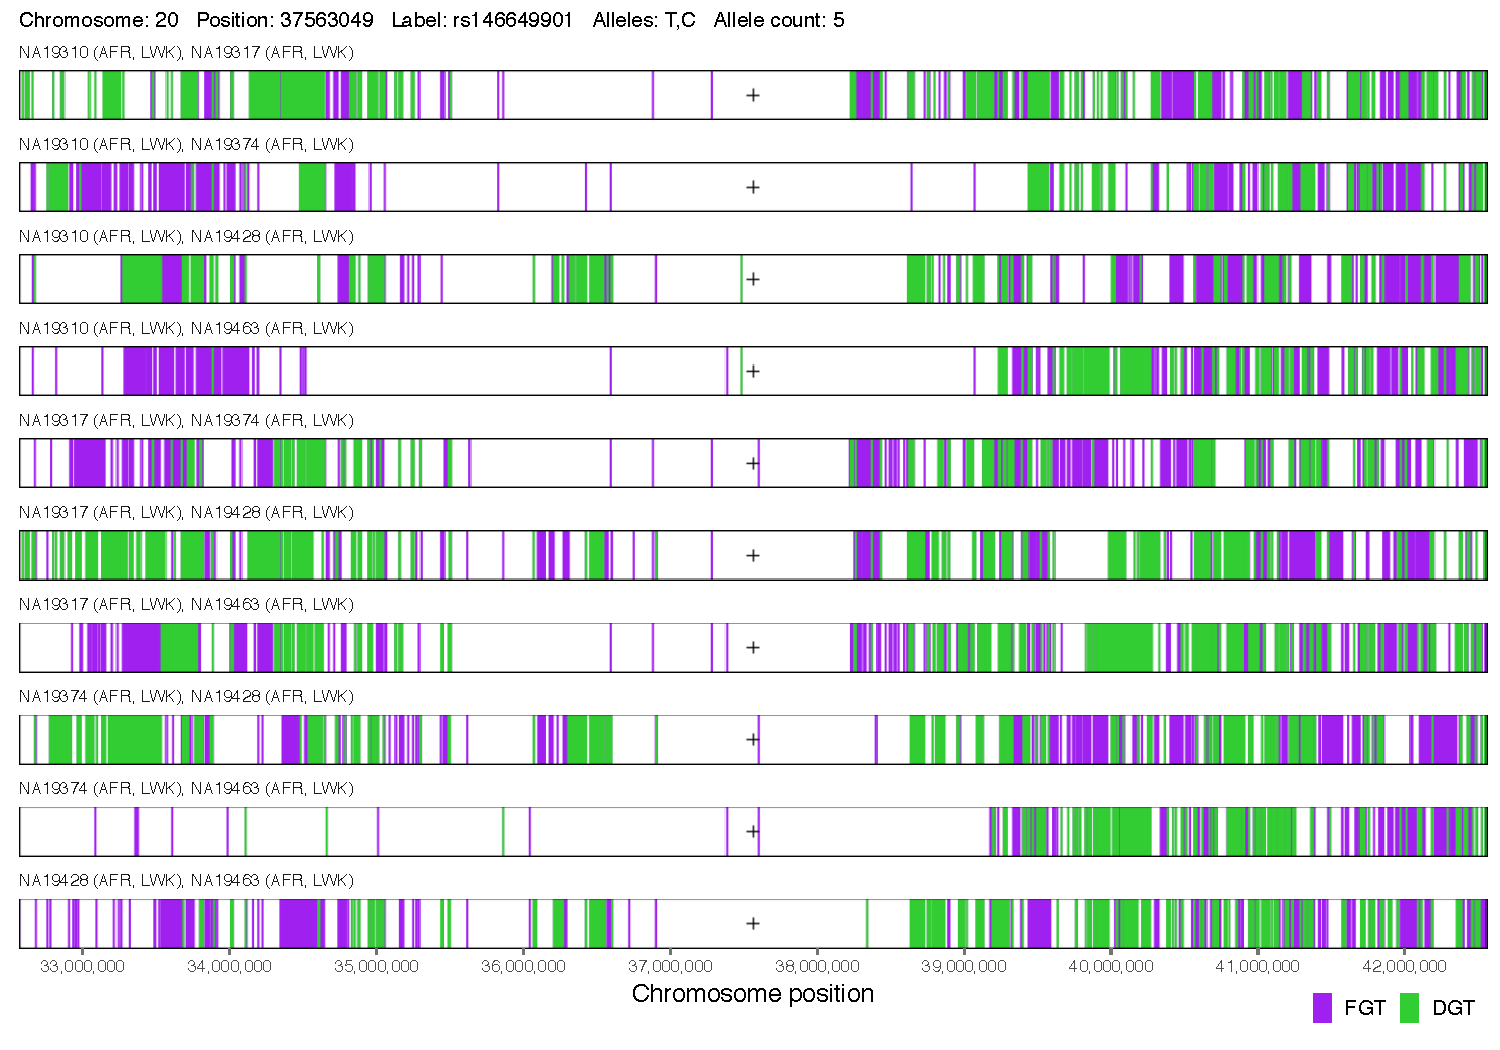
\includegraphics[width=\textwidth]{./img/ch3/ibd_example_1000G}
\Caption{Example of breakpoints detected in 1000 Genomes, chr.~20}
{One of the target sites analysed was randomly selected and breakpoint detection was performed for all pairs of individuals sharing the focal allele.
The plot shows all breakpoints detected using the \gls{fgt} and \gls{dgt} relative to the allelic configuration observed at the target site (\emph{cross}), within a \SI{10}{\mega\basepair} region around the target position.
Sample IDs (and population codes) as found in 1000 Genomes data are shown on the top of each pairwise analysis.
Note that any breakpoint detected using the \gls{dgt} also implies detection through the \gls{fgt}.}
{fig:ibd_example_1000G}
\end{figure}
